\documentclass[11pt]{standalone}
\usepackage[usenames]{color} %used for font color
\usepackage{amssymb} %maths
\usepackage{amsmath} %maths

\usepackage[no-math]{fontspec}
\usepackage{unicode-math}
\usepackage{libertinus}

\usepackage{pgf,xcolor}
\definecolor{itwm_blue_04}{HTML}{005A94}
\definecolor{itwm_red}{HTML}{C00000}
\definecolor{itwm_yellow}{HTML}{FFEC7F}

\usepackage{tikz}
\usetikzlibrary{shapes.misc, shadows, decorations, arrows}
\usetikzlibrary{backgrounds}
\usetikzlibrary{calc}
\usepackage{pgfplots}
\pgfplotsset{compat=newest}
\usepgfplotslibrary{fillbetween}
\usepackage{tikzpagenodes}

\begin{document}
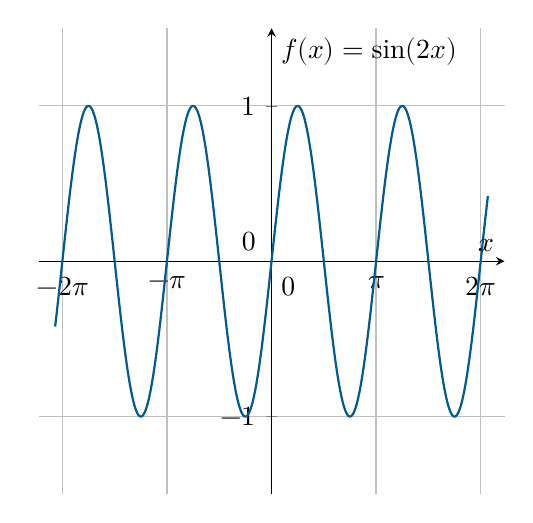
\begin{tikzpicture}
\begin{axis}[
    domain=-6.5:6.5,
    axis lines = center,
    xlabel = {$x$},
    ylabel = {$f(x)= \sin(2x)$},
    height=7.5cm, width=7.5cm, 
    xmin=-7, xmax=7, ymin=-1.5, ymax=1.5, 
    ytick={-1,0,1},
    xtick={-6.28, -3.14,...,6.28},
    xticklabels={$-2\pi$, $-\pi$, $0$, $\pi$, $2\pi$},
    grid = both,
    after end axis/.code={
        \path (axis cs:0,0) 
            node [anchor=north west,yshift=-0.075cm] {0}
            node [anchor=south east,xshift=-0.075cm] {0};
    }
]
\path [name path=xaxis]
      (\pgfkeysvalueof{/pgfplots/xmin},0) --
      (\pgfkeysvalueof{/pgfplots/xmax},0);
\addplot[draw=itwm_blue_04, smooth, thick, name path=f, samples=501]{sin(2*deg(x))};
\end{axis}
\end{tikzpicture}
%
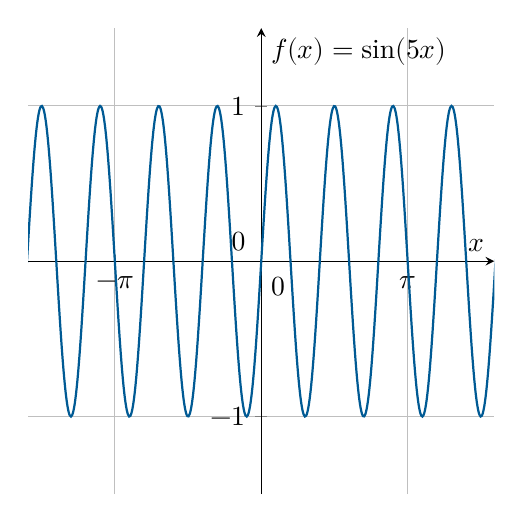
\begin{tikzpicture}
\begin{axis}[
    domain=-6.5:6.5,
    axis lines = center,
    xlabel = {$x$},
    ylabel = {$f(x)= \sin(5x)$},
    height=7.5cm, width=7.5cm, 
    xmin=-5, xmax=5, ymin=-1.5, ymax=1.5, 
    ytick={-1,0,1},
    xtick={-6.28, -3.14,...,6.28},
    xticklabels={$-2\pi$, $-\pi$, $0$, $\pi$, $2\pi$},
    grid = both,
    after end axis/.code={
        \path (axis cs:0,0) 
            node [anchor=north west,yshift=-0.075cm] {0}
            node [anchor=south east,xshift=-0.075cm] {0};
    }
]
\path [name path=xaxis]
      (\pgfkeysvalueof{/pgfplots/xmin},0) --
      (\pgfkeysvalueof{/pgfplots/xmax},0);
\addplot[draw=itwm_blue_04, smooth, thick, name path=f, samples=501]{sin(5*deg(x))};
\end{axis}
\end{tikzpicture}
%
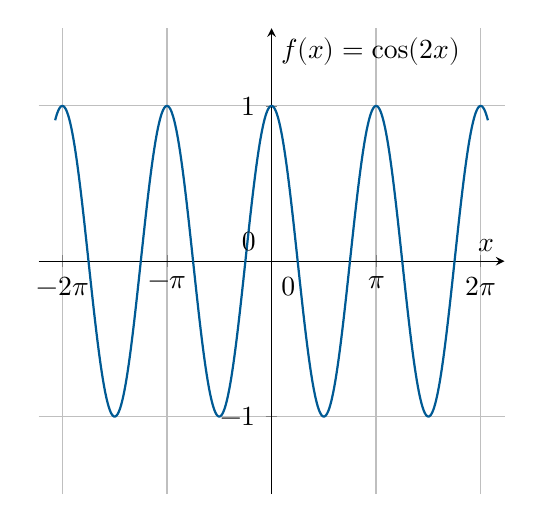
\begin{tikzpicture}
\begin{axis}[
    domain=-6.5:6.5,
    axis lines = center,
    xlabel = {$x$},
    ylabel = {$f(x)= \cos(2x)$},
    height=7.5cm, width=7.5cm, 
    xmin=-7, xmax=7, ymin=-1.5, ymax=1.5, 
    ytick={-1,0,1},
    xtick={-6.28, -3.14,...,6.28},
    xticklabels={$-2\pi$, $-\pi$, $0$, $\pi$, $2\pi$},
    grid = both,
    after end axis/.code={
        \path (axis cs:0,0) 
            node [anchor=north west,yshift=-0.075cm] {0}
            node [anchor=south east,xshift=-0.075cm] {0};
    }
]
\path [name path=xaxis]
      (\pgfkeysvalueof{/pgfplots/xmin},0) --
      (\pgfkeysvalueof{/pgfplots/xmax},0);
\addplot[draw=itwm_blue_04, smooth, thick, name path=f, samples=501]{cos(2*deg(x))};
\end{axis}
\end{tikzpicture}
%
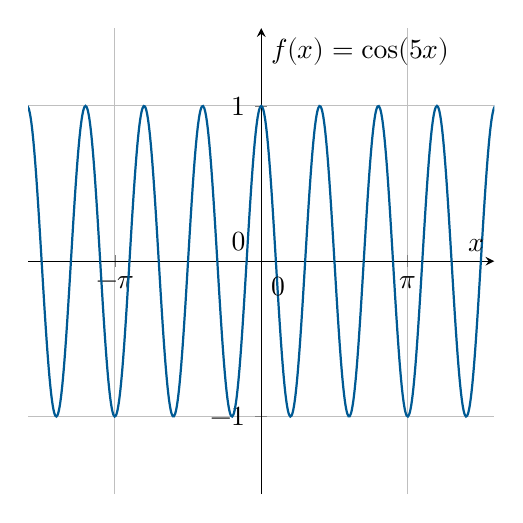
\begin{tikzpicture}
\begin{axis}[
    domain=-6.5:6.5,
    axis lines = center,
    xlabel = {$x$},
    ylabel = {$f(x)= \cos(5x)$},
    height=7.5cm, width=7.5cm, 
    xmin=-5, xmax=5, ymin=-1.5, ymax=1.5, 
    ytick={-1,0,1},
    xtick={-6.28, -3.14,...,6.28},
    xticklabels={$-2\pi$, $-\pi$, $0$, $\pi$, $2\pi$},
    grid = both,
    after end axis/.code={
        \path (axis cs:0,0) 
            node [anchor=north west,yshift=-0.075cm] {0}
            node [anchor=south east,xshift=-0.075cm] {0};
    }
]
\path [name path=xaxis]
      (\pgfkeysvalueof{/pgfplots/xmin},0) --
      (\pgfkeysvalueof{/pgfplots/xmax},0);
\addplot[draw=itwm_blue_04, smooth, thick, name path=f, samples=501]{cos(5*deg(x))};
\end{axis}
\end{tikzpicture}
\end{document}